\documentclass[tikz,border=4pt]{standalone}
\usepackage{ctex}
\usepackage{amsmath}
\usepackage{pgfplots}
\pgfplotsset{compat=1.18}

% p10-05a: 二次函数应用——面积最大（矩形面积问题示意）
% 半周长10的矩形，宽x，长10-x，面积y=x(10-x)=-x^2+10x，顶点(5,25)
\begin{document}
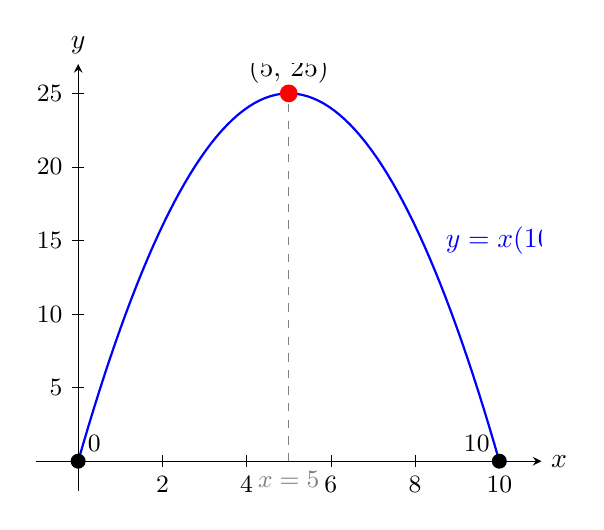
\begin{tikzpicture}
\begin{axis}[
  width=8cm, height=7cm,
  axis lines=center,
  xlabel={$x$},
  ylabel={$y$},
  every axis x label/.style={at={(axis cs:11,0)}, anchor=west},
  every axis y label/.style={at={(axis cs:0,27)}, anchor=south},
  xmin=-1, xmax=11,
  ymin=-2, ymax=27,
  xtick={2,4,6,8,10},
  ytick={5,10,15,20,25},
  tick style={color=black},
  ticklabel style={font=\small},
  clip=true,
]
  % y = -x^2 + 10x = -(x-5)^2 + 25
  \addplot[blue, thick, domain=0:10, samples=80] {-x^2+10*x};
  \node[right, blue] at (axis cs:8.5, 15) {$y=x(10-x)$};

  % 顶点 (5, 25)
  \addplot[only marks, mark=*, mark size=3pt, red] coordinates {(5,25)};
  \node[above] at (axis cs:5,25) {$(5,\,25)$};

  % 对称轴
  \draw[gray, dashed] (axis cs:5,0) -- (axis cs:5,25);
  \node[below, gray] at (axis cs:5,0) {\small$x=5$};

  % 零点
  \addplot[only marks, mark=*, mark size=2.5pt] coordinates {(0,0) (10,0)};
  \node[above right] at (axis cs:0,0) {\small$0$};
  \node[above left] at (axis cs:10,0) {\small$10$};
\end{axis}
\end{tikzpicture}
\end{document}
